\documentclass{article}\usepackage[]{graphicx}\usepackage[]{xcolor}
% maxwidth is the original width if it is less than linewidth
% otherwise use linewidth (to make sure the graphics do not exceed the margin)
\makeatletter
\def\maxwidth{ %
  \ifdim\Gin@nat@width>\linewidth
    \linewidth
  \else
    \Gin@nat@width
  \fi
}
\makeatother

\definecolor{fgcolor}{rgb}{0.345, 0.345, 0.345}
\newcommand{\hlnum}[1]{\textcolor[rgb]{0.686,0.059,0.569}{#1}}%
\newcommand{\hlstr}[1]{\textcolor[rgb]{0.192,0.494,0.8}{#1}}%
\newcommand{\hlcom}[1]{\textcolor[rgb]{0.678,0.584,0.686}{\textit{#1}}}%
\newcommand{\hlopt}[1]{\textcolor[rgb]{0,0,0}{#1}}%
\newcommand{\hlstd}[1]{\textcolor[rgb]{0.345,0.345,0.345}{#1}}%
\newcommand{\hlkwa}[1]{\textcolor[rgb]{0.161,0.373,0.58}{\textbf{#1}}}%
\newcommand{\hlkwb}[1]{\textcolor[rgb]{0.69,0.353,0.396}{#1}}%
\newcommand{\hlkwc}[1]{\textcolor[rgb]{0.333,0.667,0.333}{#1}}%
\newcommand{\hlkwd}[1]{\textcolor[rgb]{0.737,0.353,0.396}{\textbf{#1}}}%
\let\hlipl\hlkwb

\usepackage{framed}
\makeatletter
\newenvironment{kframe}{%
 \def\at@end@of@kframe{}%
 \ifinner\ifhmode%
  \def\at@end@of@kframe{\end{minipage}}%
  \begin{minipage}{\columnwidth}%
 \fi\fi%
 \def\FrameCommand##1{\hskip\@totalleftmargin \hskip-\fboxsep
 \colorbox{shadecolor}{##1}\hskip-\fboxsep
     % There is no \\@totalrightmargin, so:
     \hskip-\linewidth \hskip-\@totalleftmargin \hskip\columnwidth}%
 \MakeFramed {\advance\hsize-\width
   \@totalleftmargin\z@ \linewidth\hsize
   \@setminipage}}%
 {\par\unskip\endMakeFramed%
 \at@end@of@kframe}
\makeatother

\definecolor{shadecolor}{rgb}{.97, .97, .97}
\definecolor{messagecolor}{rgb}{0, 0, 0}
\definecolor{warningcolor}{rgb}{1, 0, 1}
\definecolor{errorcolor}{rgb}{1, 0, 0}
\newenvironment{knitrout}{}{} % an empty environment to be redefined in TeX

\usepackage{alltt}
\usepackage[]{graphicx}
\usepackage[]{color}

\title{Deploying the RPi and AQ Sensors}
\author{Marc Los Huertos}
\IfFileExists{upquote.sty}{\usepackage{upquote}}{}
\begin{document}
\maketitle

\section{Introduction}

\subsection{How is particulate matter ``sampled''?}

The PM sensor has several components to measure the particles in the air -- remember, we don't know what the make up of these particles might be -- but we can get an estimate of their size distribution. We have written the code to collect particles smaller than 1$\mu$m, 2.5$\mu$m and 10$\mu$m. 

Figure~\ref{fig:hpsensor} is a schematic of the particle sensor made by Honeywell (HPM Series --- Particulate Matter Sensors 32322550HP). The one we are using is made by Plantower. As a Chinese company, most of their literature is in Chinese, so I didn't find something that I could interpret for us. 

\begin{figure}
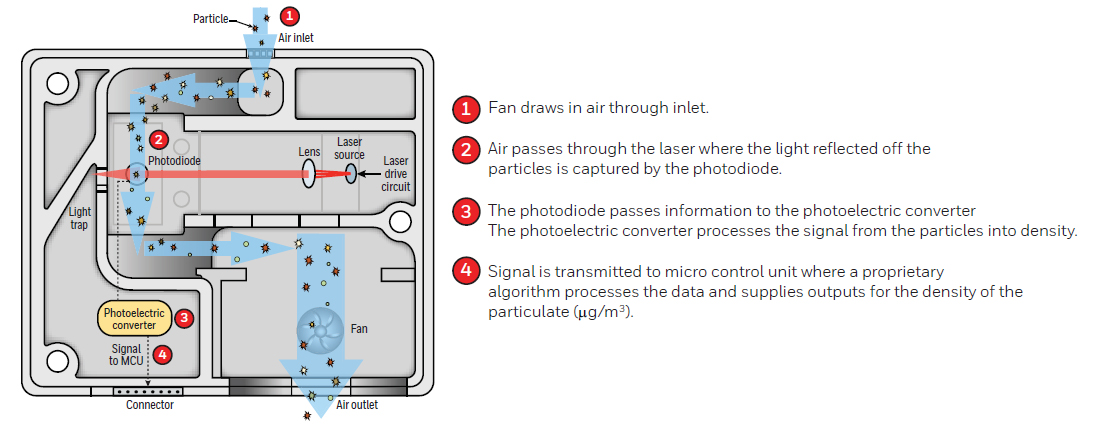
\includegraphics[width=1.00\textwidth]{images/4_SensorSchematic}
\caption{Schematic of Honeywell Particulate Matter Sensor. A laser light source illuminates a particle as it is pulled through the detection chamber. As particles pass through the laser beam, the light reflects off the particles and is recorded on the photo or light detector. The light is then analyzed and converted to an electrical signal to calculate particle concentration.}
\label{fig:hpsensor}
\end{figure}

Our sensors can generate several categories of PM data. Using a laser and light defraction, the number and size of the particles can be estimated (Figure~\ref{fig:defraction}).

\begin{figure}
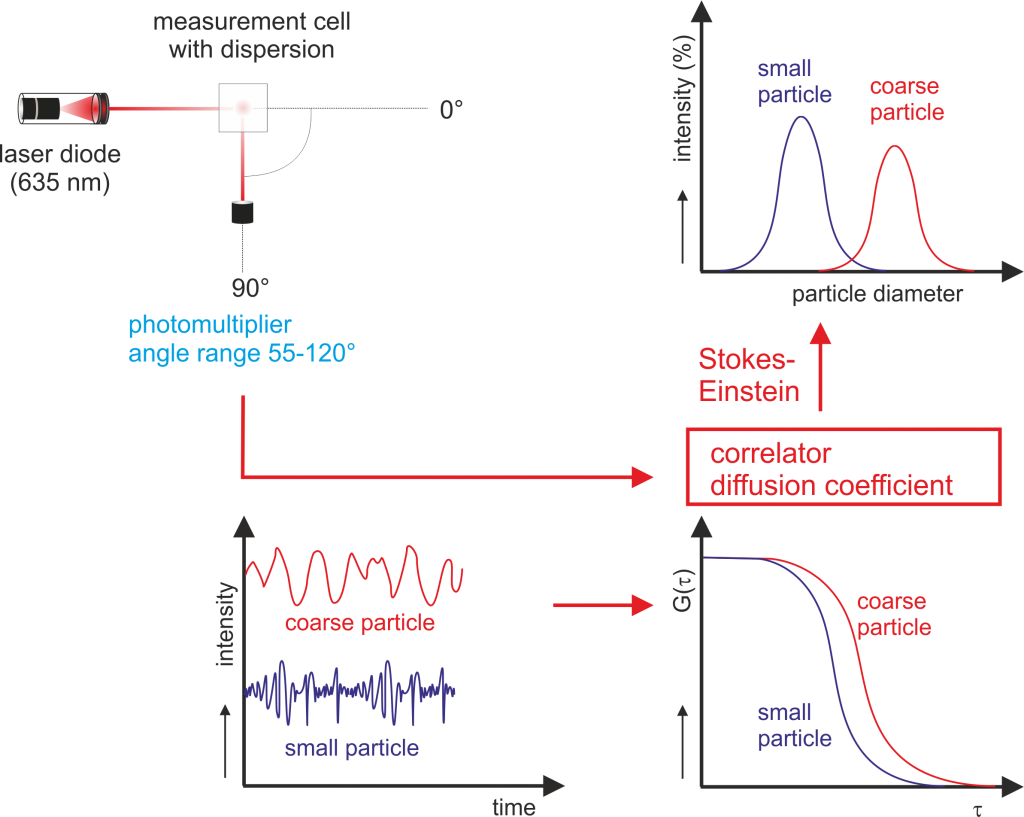
\includegraphics[width=0.70\textwidth]{images/4_Measurement-principle}
\caption{In particle size measurements using light scattering (DLS), a laser beam is scattered on very small, finely dispersed particles in a highly diluted matrix. 
The scattered light of each particle will then interfere with each other. Since the particles constantly change locations, the position of the scattering centers changes with respect to each other and the interferences lead to small fluctuations in scattering intensity (this explains the name ``dynamic'' light scattering).}
\label{fig:defraction}
\end{figure}

\subsection{Developing a Reasonable Question}

As defined in your prospectus, we need to ensure our research question aligns with our methods -- and our analysis prodedures, which is often a statistical test. 

\subsection{Testing Methods}

One effective way do to this is to collect preliminary data to ensure we will get reasonable results. 

\subsection{Creating Reliable Data Sources}

\section{Deploying the Pis}

We did not have the capacity to create a robust case for our Pis that might allow them to be deployed without exposure to the elements. 

Thus, here are some suggestions:

\begin{itemize}
  \item Put the Pi and breadboard in a plastic sandwich bad and/or tupperware container. Make holes for the power input and the can PM sensor cable. 
  \item Put the sensor at where there is good air flow outside a wondow that you can provide power to the Pi. Or better yet, find a location outide where a power socket is available.  Note: the cable switch is not water proof, so be to protect the on/off switch; maybe put in a plastic bag too?
  \item Hopefully, the Pi still connects to your WiFi. If not, we'll have to come up with a method to launch the program on boot up. Work with Kyle if you have this issue, breifly we will 
  
\begin{itemize}
  \item Edit the rc.local file to include the path of your script that you want to run. In our case, it's whatever python file. The rc.local file is located at /etc/rc.local in nearly every Linux distribution. YES, the Pi's OS is Linux.
  \item Modify the Pi Configuration Utility and change the Boot option to: ``Boot To CLI''. That way, the next boot, it boots to the command line interface and runs the python script and if the program is a loop it'll keep running the script until you exit it.
  
\end{itemize}


\end{itemize}


\section{Collecting the data}

Once the data have been collected, you can extract the data from the SD card and copy to r for processing. 

\subsection{Processing the data}

Marc will be creating a script to process the data and allow you to create a nice dataframe to analyze the data.

\begin{knitrout}
\definecolor{shadecolor}{rgb}{0.969, 0.969, 0.969}\color{fgcolor}\begin{kframe}
\begin{alltt}
\hlstd{filepath.csv} \hlkwb{=} \hlstr{"/home/CAMPUS/mwl04747/github/EJnPi/data/TestData.R"}
\hlstd{rawdata} \hlkwb{=} \hlkwd{read.csv}\hlstd{(filepath.csv)}
\end{alltt}


{\ttfamily\noindent\color{warningcolor}{\#\# Warning in file(file, "{}rt"{}): cannot open file '/home/CAMPUS/mwl04747/github/EJnPi/data/TestData.R': No such file or directory}}

{\ttfamily\noindent\bfseries\color{errorcolor}{\#\# Error in file(file, "{}rt"{}): cannot open the connection}}\end{kframe}
\end{knitrout}

\end{document}
